\documentclass[sn-mathphys-num]{sn-jnl}
%% The project bundle includes a lightweight sn-jnl.cls compatibility shim so
%% this manuscript can compile in a clean Overleaf project. For a journal
%% submission, replace the shim with the official Springer Nature class files.

\usepackage{booktabs}
\usepackage{graphicx}
\usepackage{amsmath,amssymb}
\usepackage{array,multirow}
\usepackage{siunitx}
\usepackage{placeins}
\usepackage{enumitem}
\usepackage{xcolor}
\usepackage{float}
\usepackage[colorlinks=true,linkcolor=black,citecolor=black,urlcolor=blue!55!black]{hyperref}
\usepackage[capitalise,noabbrev]{cleveref}
\usepackage{orcidlink}

\geometry{a4paper,left=4cm,right=4cm,top=2.45cm,bottom=2.45cm}
\raggedbottom

\graphicspath{{figures/}{../figures/}}
\setkeys{Gin}{draft=false}
\sisetup{detect-all,group-minimum-digits=4}
\setlength{\textfloatsep}{6pt plus 2pt minus 2pt}
\setlength{\floatsep}{5pt plus 2pt minus 2pt}
\setlength{\intextsep}{5pt plus 2pt minus 2pt}
\setlength{\dbltextfloatsep}{6pt plus 2pt minus 2pt}
\setlength{\dblfloatsep}{5pt plus 2pt minus 2pt}
\setlength{\abovecaptionskip}{4pt}
\setlength{\belowcaptionskip}{2pt}
\AtBeginDocument{%
  \setlength{\abovedisplayskip}{4pt plus 1pt minus 1pt}%
  \setlength{\belowdisplayskip}{4pt plus 1pt minus 1pt}%
  \setlength{\abovedisplayshortskip}{3pt plus 1pt minus 1pt}%
  \setlength{\belowdisplayshortskip}{3pt plus 1pt minus 1pt}%
}

\definecolor{pmred}{HTML}{E4572E}
\definecolor{tmblue}{HTML}{2E86AB}
\definecolor{xgbgreen}{HTML}{2E9E5B}
\definecolor{panel}{HTML}{F4F6F8}
\definecolor{ink}{HTML}{23313F}

\newcommand{\PM}{\mathrm{PM}_{2.5}}
\newcommand{\TM}{\textsc{TimeMixer}}
\newcommand{\XGB}{\textsc{XGBoost}}
\newcommand{\HYB}{\textsc{TM-XGB}}
\newcommand{\Exp}{\mathbb{E}}
\newcommand{\Real}{\mathbb{R}}
\newcommand{\Horizons}{\{1,6,12,24,48\}}
\newcommand{\given}{\,\vert\,}
\newcommand{\smallorcid}[1]{\textnormal{\scriptsize\,(#1)}}

\title{Gated TimeMixer-XGBoost for PM2.5 Forecasting}

\author[1]{\fnm{Ngan} \sur{Pham}
\smallorcid{0009-0001-1089-2626}}
\email{tunganphamhoang@gmail.com}

\author[1]{\fnm{Nhi} \sur{Tran}
\smallorcid{0009-0001-1047-5080}}
\email{nhikl12006@gmail.com}

\author[1]{\fnm{Han} \sur{Dong}
\smallorcid{0009-0002-2532-8099}}
\email{donghan010106@gmail.com}

\author[1]{\fnm{Thu} \sur{Le}
\smallorcid{0009-0008-3480-8311}}
\email{thulvm@fpt.edu.vn}

\affil{
  \orgdiv{Faculty of Information Technology},
  \orgname{FPT University},
  \orgaddress{
    \city{Ho Chi Minh City},
    \country{Vietnam}
  }
}

\affil[]{
  \textbf{Emails:}
  \texttt{tunganphamhoang@gmail.com};
  \texttt{nhikl12006@gmail.com};
  \texttt{donghan010106@gmail.com};
  \texttt{thulvm@fpt.edu.vn}
}

\abstract{Accurate multi-horizon PM2.5 forecasting is difficult because hourly
monitoring records combine persistence, periodicity, abrupt episodes,
missing observations, site heterogeneity, and measurement-regime changes.
This study evaluates a calibration-gated TimeMixer-XGBoost framework at five
UK-Air stations and horizons of 1, 6, 12, 24, and 48 hours. The residual stage
removes calibration-period median bias, fits horizon-specific XGBoost models
with pseudo-Huber loss and bounded corrections, selects a correction scale on
a later held-out calibration subset, and applies rolling calibration using
only errors observable at each forecast origin. The benchmark includes
persistence, seasonal-naive, direct XGBoost, DLinear, LSTM, TimeMixer,
ungated robust correction, gated static correction, and gated rolling
correction. Neural experiments use seeds 0-4 and a 30-epoch maximum under
separate training, early-stopping, residual-fit, gate-selection, and
locked-test eras. The confirmatory experiment completed five stations, five seeds, and a 30-epoch maximum. The hybrid won 0/25 comparisons against the strongest matched non-hybrid comparator, giving a 23.33\% MAE gap, but improved compact TimeMixer and prevented severe ungated over-correction. LSTM (MAE 3.271) and DLinear (3.282) were practically tied; DLinear led pooled RMSE and sMAPE. Common-history sensitivity changed hybrid MAE by only \( +0.012 \), so the result is a leakage-controlled negative finding, not a state-of-the-art claim.
}

\keywords{PM2.5; TimeMixer; XGBoost; multi-horizon forecasting; air quality; residual learning; time-series forecasting; reproducibility}

\begin{document}
\maketitle
\section{Introduction}
\label{sec:intro}

Fine particulate matter (\(\PM\)) is a central air-quality indicator linked to
respiratory and cardiovascular risk \cite{who2021aqg}. For operators and public
dashboards, the useful question is not only whether pollution is high now, but
whether it will remain high over the next few hours or days. This study targets
hourly forecasts at 1, 6, 12, 24, and 48 hours.

Historical \(\PM\) forecasting is difficult because short-horizon persistence,
daily/weekly cycles, abrupt episodes, and imperfect monitoring archives occur
together. Missing observations, long outages, negative source values, and
instrument changes can make a model appear accurate if they are silently
interpolated or split randomly across training and test sets.

The paper therefore evaluates a leakage-controlled pipeline, not only a model
architecture. The proposed model uses \TM{} as a compact multiscale base and
\XGB{} as a horizon-specific residual corrector. Its conservative residual layer
removes median bias, uses pseudo-Huber loss, clips extreme corrections, selects
a non-negative held-out gate, and updates recent bias only from origin-available
errors. The practical question is whether boosted residual correction can help a
neural forecaster without creating unstable over-correction.

The empirical study uses five UK-Air stations across urban traffic, urban
background, and rural background settings. All experiments share chronological
partitions, origin-safe features, five seeds, and a 30-epoch neural budget. The
results are read against two standards: whether gating improves the compact
\TM{} base, and whether the hybrid beats the strongest matched comparator. The
experiment supports the first claim, but not the second.

This framing is important for a student research project because air-quality
forecasting can look successful if the comparison set is too weak. A model that
beats only seasonal-naive forecasts may still be less useful than a direct tree
model or a simple recurrent network. The study therefore treats persistence,
XGBoost, DLinear, and LSTM as serious competitors rather than background
baselines. It also reports station-specific data problems before modeling, so
negative source values, incomplete coverage, and instrument changes are not
hidden behind a single accuracy number.

The contributions are threefold: an auditable PM2.5-only pipeline, a
conservative residual-correction design that can abstain, and a transparent
negative finding showing that simple/recurrent baselines remain stronger while
gating teaches when hybrid correction should back off.

\section{Related Work}
\label{sec:related}

Classical methods remain relevant because air-quality series contain
persistence and calendar structure \cite{hyndman2021fpp3}. Persistence and
seasonal-naive forecasts are therefore real baselines, especially at short
horizons. PM2.5 studies also show that rankings vary with inputs, architecture,
and lead time \cite{beijing2021forecast}, motivating horizon-wise reporting.

Neural sequence models provide stronger nonlinear temporal representations.
LSTM is a common recurrent baseline for hourly PM2.5 forecasting
\cite{hochreiter1997lstm,bai2019ensemble}. More recent long-horizon models
represent temporal structure through decomposition, patches, or multiscale
mixing, including N-BEATS \cite{oreshkin2020nbeats}, PatchTST
\cite{nie2023patchtst}, DLinear \cite{zeng2023dlinear}, Temporal Fusion
Transformers \cite{lim2021temporal}, and TimeMixer
\cite{wang2024timemixer}. TimeMixer is especially relevant here because it
mixes information across downsampled temporal scales, which matches the
coexistence of short-lag persistence and slower pollution cycles.

Tree ensembles offer a complementary advantage. XGBoost efficiently models
interactions among lags, rolling statistics, calendar variables, and
measurement-regime indicators \cite{chen2016xgboost}; related systems such as
LightGBM show the strength of boosted trees on structured data
\cite{ke2017lightgbm}. Here, XGBoost corrects TimeMixer residuals under the
direct multi-step view that different horizons may need different error models
\cite{taieb2012review}.

Evaluation must respect temporal dependence: random splits can leak
near-duplicate contexts across train and test \cite{bergmeir2018cv}. This study
therefore uses chronological partitions, origin-safe features, MAE
\cite{willmott2005mae}, paired evidence \cite{diebold1995accuracy,newey1987hac},
and SHAP only as predictive diagnostics \cite{lundberg2017shap}. Because
residual tuning can otherwise learn test-specific bias, neural validation,
residual fitting, gate selection, and locked testing are separated.

A further issue in hybrid forecasting is that residual learners can easily
overfit the remaining error of a base model. If the base forecast is already
biased or noisy, a second-stage learner may amplify rather than correct the
mistake. This motivates the conservative design used in this paper: residual
correction is treated as optional calibration, not as an automatic performance
boost. The gate is selected on calibration data only, and the model is allowed
to return to the original TimeMixer forecast when correction evidence is weak.

\section{Method}
\label{sec:method}

The method combines data cleaning, origin-safe feature construction,
multi-horizon neural forecasting, residual calibration, and locked evaluation.
The goal is to preserve the evidence trail from raw monitoring records while
preventing future information from entering model inputs.

\begin{figure}[!t]
\vspace{-4pt}
\centering
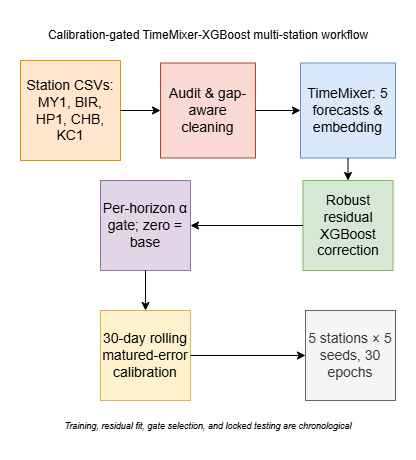
\includegraphics[draft=false,width=0.62\linewidth]{00_framework.png}
\caption{End-to-end framework: TimeMixer generates base forecasts, and a later calibration interval fits and gates residual XGBoost before locked testing.}
\vspace{-8pt}
\label{fig:framework}
\end{figure}

\subsection{Data and monitoring stations}
\label{sec:site}

The confirmatory dataset contains five UK-Air stations selected to represent
different monitoring environments: London Marylebone Road (MY1, urban
traffic), Birmingham A4540 (BIR\_A4540, urban traffic), London Honor Oak Park
(HP1, urban background), Chilbolton (CHB, rural background), and London North
Kensington (KC1, urban background). Marylebone Road is a well-studied urban
roadside site \cite{kamara2021marylebone}, and UK-Air metadata are used to
verify station identity and monitoring context
\cite{ukair2026my1,ukair2026kc1,ukair2026hp1}. Each station is processed
independently with the same schema, cleaning rules, forecast horizons,
chronological boundaries, seeds, and evaluation metrics. Dataset paths and
site types are fixed in \texttt{data/stations.csv}.

UK-Air provides the date and hour-ending time in separate fields. During ingestion, the pipeline combines these fields while retaining the original filename, row identifier, timestamp and concentration values, along with the associated status information. A source time of 24:00 is
normalized to 00:00 of the following day. The target is hourly PM2.5 mass
concentration in \si{\micro\gram\per\cubic\meter}.

\begin{table}[tbp]
\centering
\caption{Station-specific data limitations identified before model fitting.}
\label{tab:station-quality}
\footnotesize
\begin{tabular}{p{0.13\linewidth}p{0.18\linewidth}p{0.34\linewidth}p{0.25\linewidth}}
\toprule
Station & Type & Available-history issue & Pre-specified treatment \\
\midrule
MY1 & Urban traffic & 2020 coverage 77.81\%; 69-day gap & Preserve long gap; reject affected windows \\
BIR\_A4540 & Urban traffic & Record begins in 2021 & Report shorter training history \\
HP1 & Urban background & No observations in 2016-2018 & Treat as unavailable, not imputed \\
CHB & Rural background & 2024 coverage 73.44\%; 561 negatives & Mask negatives; preserve unresolved gaps \\
KC1 & Urban background & Instrument-regime transition & Retain instrument type as context \\
\bottomrule
\end{tabular}
\end{table}

These differences imply unequal training histories. The primary analysis uses
each station's available archive, while a common-history sensitivity run
restricts all stations to records from 2021 onward.

\subsection{Auditable cleaning}
\label{sec:cleaning}

The raw file is immutable. Cleaning separates \emph{raw} source evidence,
\emph{observed} non-negative measurements, and \emph{clean} values with only
approved short-gap interpolation. Row flags record invalid timestamps, missing
or negative values, duplicates, inserted grid rows, interpolation, and long gaps.

Linear interpolation is allowed only for internal gaps no longer than three
hours. Longer gaps remain missing, and any model window crossing unresolved
missingness is rejected. Instrument information is parsed from source status
metadata and encoded as TEOM FDMS \(=0\) and BAM \(=1\), because measurement
regime can alter the statistical distribution even when it is not causal.

\begin{table}[tbp]
\centering
\caption{Verified quality profile of the supplied London Marylebone Road record.}
\label{tab:dataaudit}
\small
\begin{tabular}{lr}
\toprule
Audit item & Value \\
\midrule
Raw hourly rows & \num{87672} \\
Missing/non-numeric readings & \num{8087} \\
Negative numeric measurements & \num{238} \\
Longest invalid run & \num{1656} h (69 d) \\
2020 valid coverage after negative exclusion & 77.81\% \\
Instrument transition & 22 Dec 2021, 12:00 UTC \\
Primary short-gap interpolation limit & 3 h \\
\bottomrule
\end{tabular}
\end{table}

\subsection{Origin-safe predictors}
\label{sec:originsafe}

Predictors include calendar encodings, PM2.5 lags at 1--168 hours, shifted
rolling summaries, differences, and instrument type. Every rolling summary is
shifted by one hour, so features at origin \(t\) contain values no later than
\(t-1\); \(y_t\) remains available as the last sequence value.

Rather than presenting origin safety as a formal theorem, we enforce it as a core pipeline rule. All sequence, lag, rolling, calendar, instrument, and missingness features must be available by the forecast origin \(t\). In contrast, target values must occur strictly after \(t\) and remain within their designated chronological partition.
 This matters because multi-horizon windows
overlap heavily. A random split would place nearly identical contexts on both
sides of a boundary, whereas chronological partitions preserve the information
set available at deployment.

\subsection{SQL-style and Python analysis}
\label{sec:query-analysis}

Python scripts generate the evidence, and SQL-style grouped queries organize
comparisons by station, horizon, model, seed, and experiment setting. Model
ranking answers RQ1, TimeMixer-versus-hybrid joins answer RQ2, and
available-history versus common-2021 joins answer RQ3.

\subsection{Forecasting task}
\label{sec:problem}

Let \(y_t\) denote hourly PM2.5. Each model uses the previous 168 hours as an
origin-available multichannel sequence containing cleaned PM2.5, a missingness
mask, instrument type, and cyclic calendar encodings. For horizon set
\(\mathcal H=\Horizons\), the direct task is
\begin{equation}
\hat{\mathbf y}_t=
\left(\hat y_{t+1},\hat y_{t+6},\hat y_{t+12},\hat y_{t+24},\hat y_{t+48}\right).
\end{equation}
Predictions are generated simultaneously and are not recursively fed back.
Direct prediction avoids recursive error accumulation and permits one residual
correction function per horizon.

\subsection{TimeMixer base forecaster}
\label{sec:timemixer}

The implementation is a compact research adaptation of TimeMixer's multiscale
ideas rather than a line-for-line reproduction of the official benchmark code
\cite{wang2024timemixer}. The 168-hour input is downsampled across several
scales, decomposed into smooth and residual components, mixed by MLP blocks,
and mapped to the five forecast horizons. The learned multiscale embedding is
also reused by residual XGBoost. Huber loss, AdamW, gradient clipping, and
early stopping are used; input and target standardizers are fitted on training
windows only.

\subsection{Gated residual XGBoost}
\label{sec:residual}

The residual-calibration interval is split chronologically into residual-fit
(70\%) and gate-selection (30\%) subsets. For each horizon, the residual is
median-centred, learned by a robust XGBoost model, clipped to calibration
quantiles, and scaled by a held-out gate:
\begin{equation}
\hat y^{HYB}_{t,h}
=\hat y^{TM}_{t,h}
+\gamma_h\hat c_{t,h}
+\lambda_t\,\operatorname{median}(\mathcal E_{t,h}).
\end{equation}
Here \(\gamma_h\in\{0,0.10,0.25,0.50,0.75,1\}\) is selected on the later
calibration subset, so \(\gamma_h=0\) can fall back to TimeMixer when correction
does not improve calibration MAE. The context vector contains origin-safe lags,
shifted rolling features, instrument type, calendar variables, missingness
state, gap length, interpolation status, measurement-quality flags, the full
base forecast vector, and the latent embedding. Each residual booster uses
pseudo-Huber loss, row/feature subsampling, \(L_1/L_2\) regularization, and a
rolling 30-day error set whose target timestamps are no later than origin \(t\).

\subsection{Experimental setup}
\label{sec:setup}

Four consecutive eras separate fitting, early stopping, residual calibration,
and locked testing. Historical context may cross a boundary, but forecast
targets must remain inside their assigned partition.

\begin{table}[tbp]
\centering
\caption{Temporal partitions and permitted use.}
\label{tab:splits}
\small
\begin{tabular}{p{0.22\linewidth}p{0.31\linewidth}p{0.37\linewidth}}
\toprule
Partition & Period & Permitted use \\
\midrule
Training & through 31 Dec 2022 & scalers; neural weights; direct XGBoost \\
Neural validation & 1 Jan-31 Dec 2023 & early stopping only \\
Hybrid calibration & 1 Jan-30 Jun 2024 & residual fit (first 70\%); gate selection (last 30\%) \\
Locked test & after 30 Jun 2024 & final paired evaluation only \\
\bottomrule
\end{tabular}
\end{table}

Comparators are persistence, seasonal-naive, direct XGBoost,
DLinear~\cite{zeng2023dlinear}, LSTM, and TimeMixer. Static and rolling hybrid
variants isolate residual safeguards. Neural models use seeds 0--4, batch size
128, AdamW at \(10^{-3}\), early-stopping patience seven, and at most 30
epochs. MAE is primary; RMSE, sMAPE, \(R^2\), bias, and fixed
training-90th-percentile event metrics are secondary. A paired bootstrap
resamples 24-hour blocks of the absolute-error difference between the hybrid
and TimeMixer; negative differences favor the hybrid. Diebold-Mariano tests
use absolute loss and Holm correction
\cite{diebold1995accuracy}. Same-origin ablations isolate embeddings, context,
gating, and rolling calibration.

\section{Results}
\label{sec:results}

The first empirical finding is that preprocessing choices materially change
the admissible forecasting sample. At MY1, the record contains 8,087 missing
or non-numeric readings, 238 negative values, and a 1,656-hour maximum invalid
run. Cross-station auditing reveals additional heterogeneity: HP1 contains no
observations in 2016-2018; BIR\_A4540 begins in 2021; CHB has only 73.44\%
coverage in 2024 and contains 561 negative source values; and KC1 contains an
instrument-regime transition. Negative PM2.5 concentrations are not interpreted as physical pollution
levels; they are treated as invalid source readings, masked from the modelling
target, and retained only as audit evidence. None of these intervals or invalid
values is reconstructed through long-range interpolation. Instead, invalid
values remain auditable and forecast windows crossing unresolved gaps are
excluded.

\IfFileExists{figures/01_data_overview.png}{
\begin{figure}[!t]
\centering
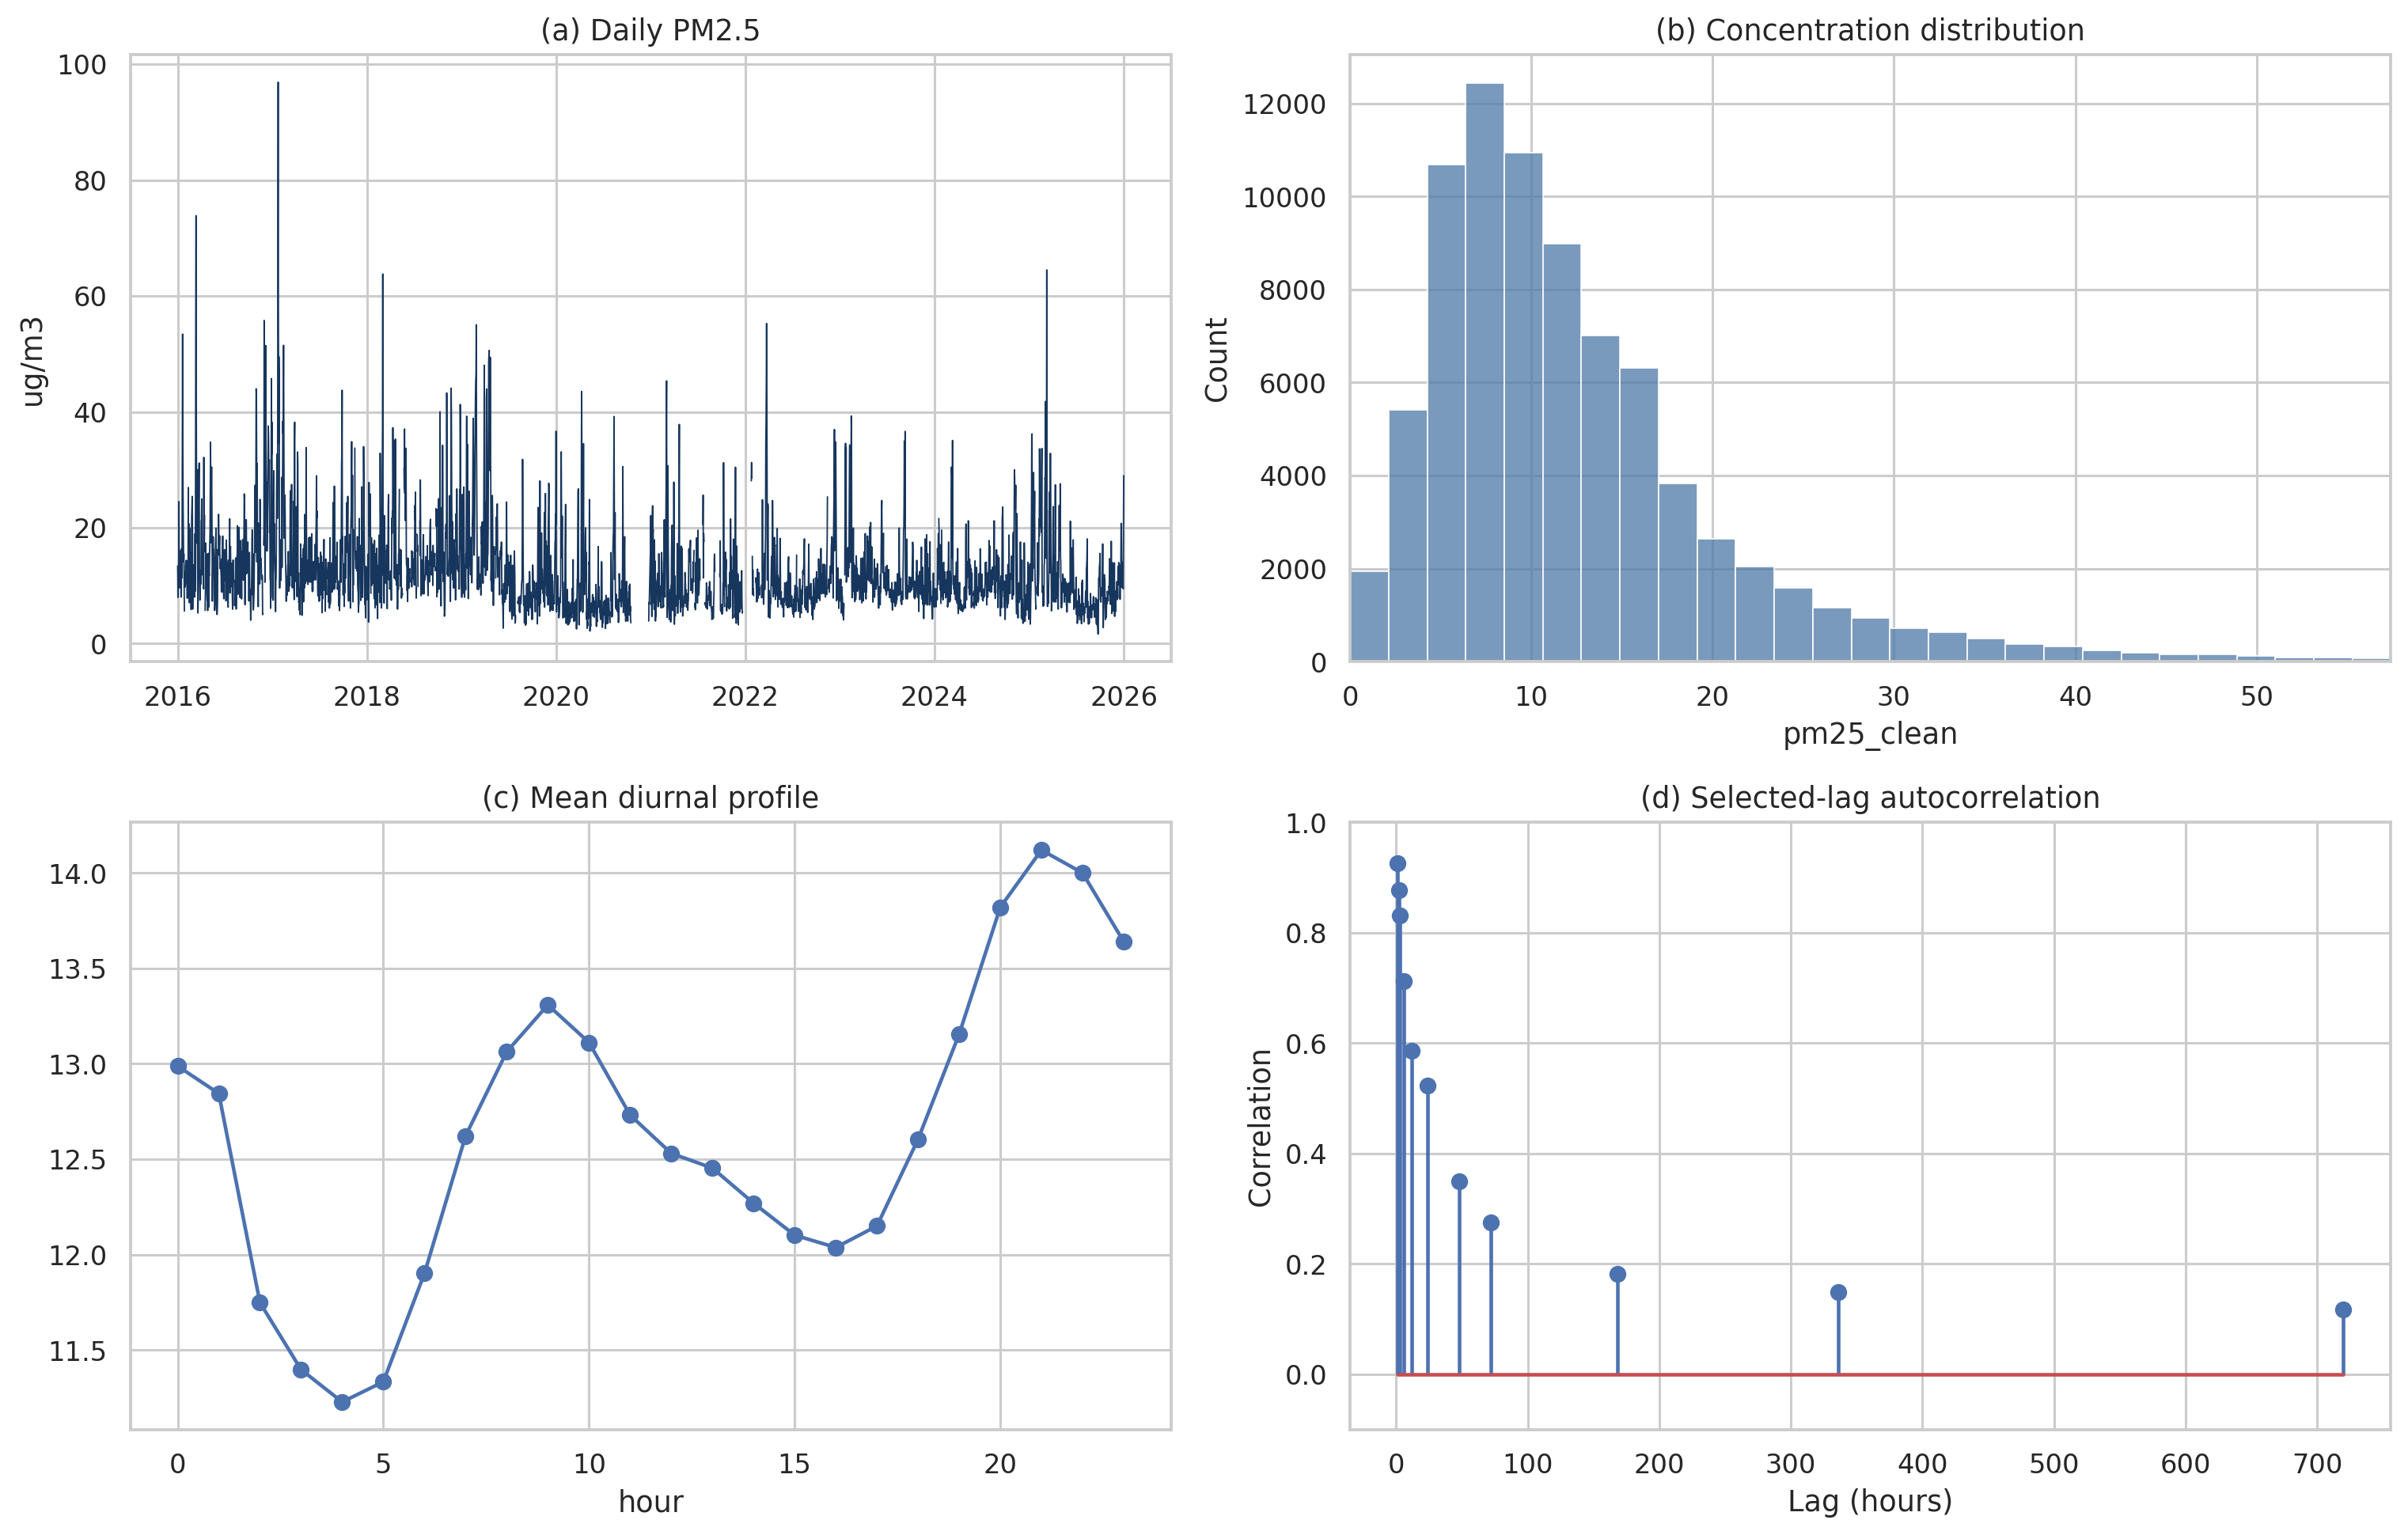
\includegraphics[width=\linewidth]{01_data_overview.png}
\caption{EDA overview: daily PM2.5, distribution, diurnal profile, and autocorrelation.}
\label{fig:data-overview}
\end{figure}}{}

\IfFileExists{figures/02_data_quality.png}{
\begin{figure}[!t]
\centering
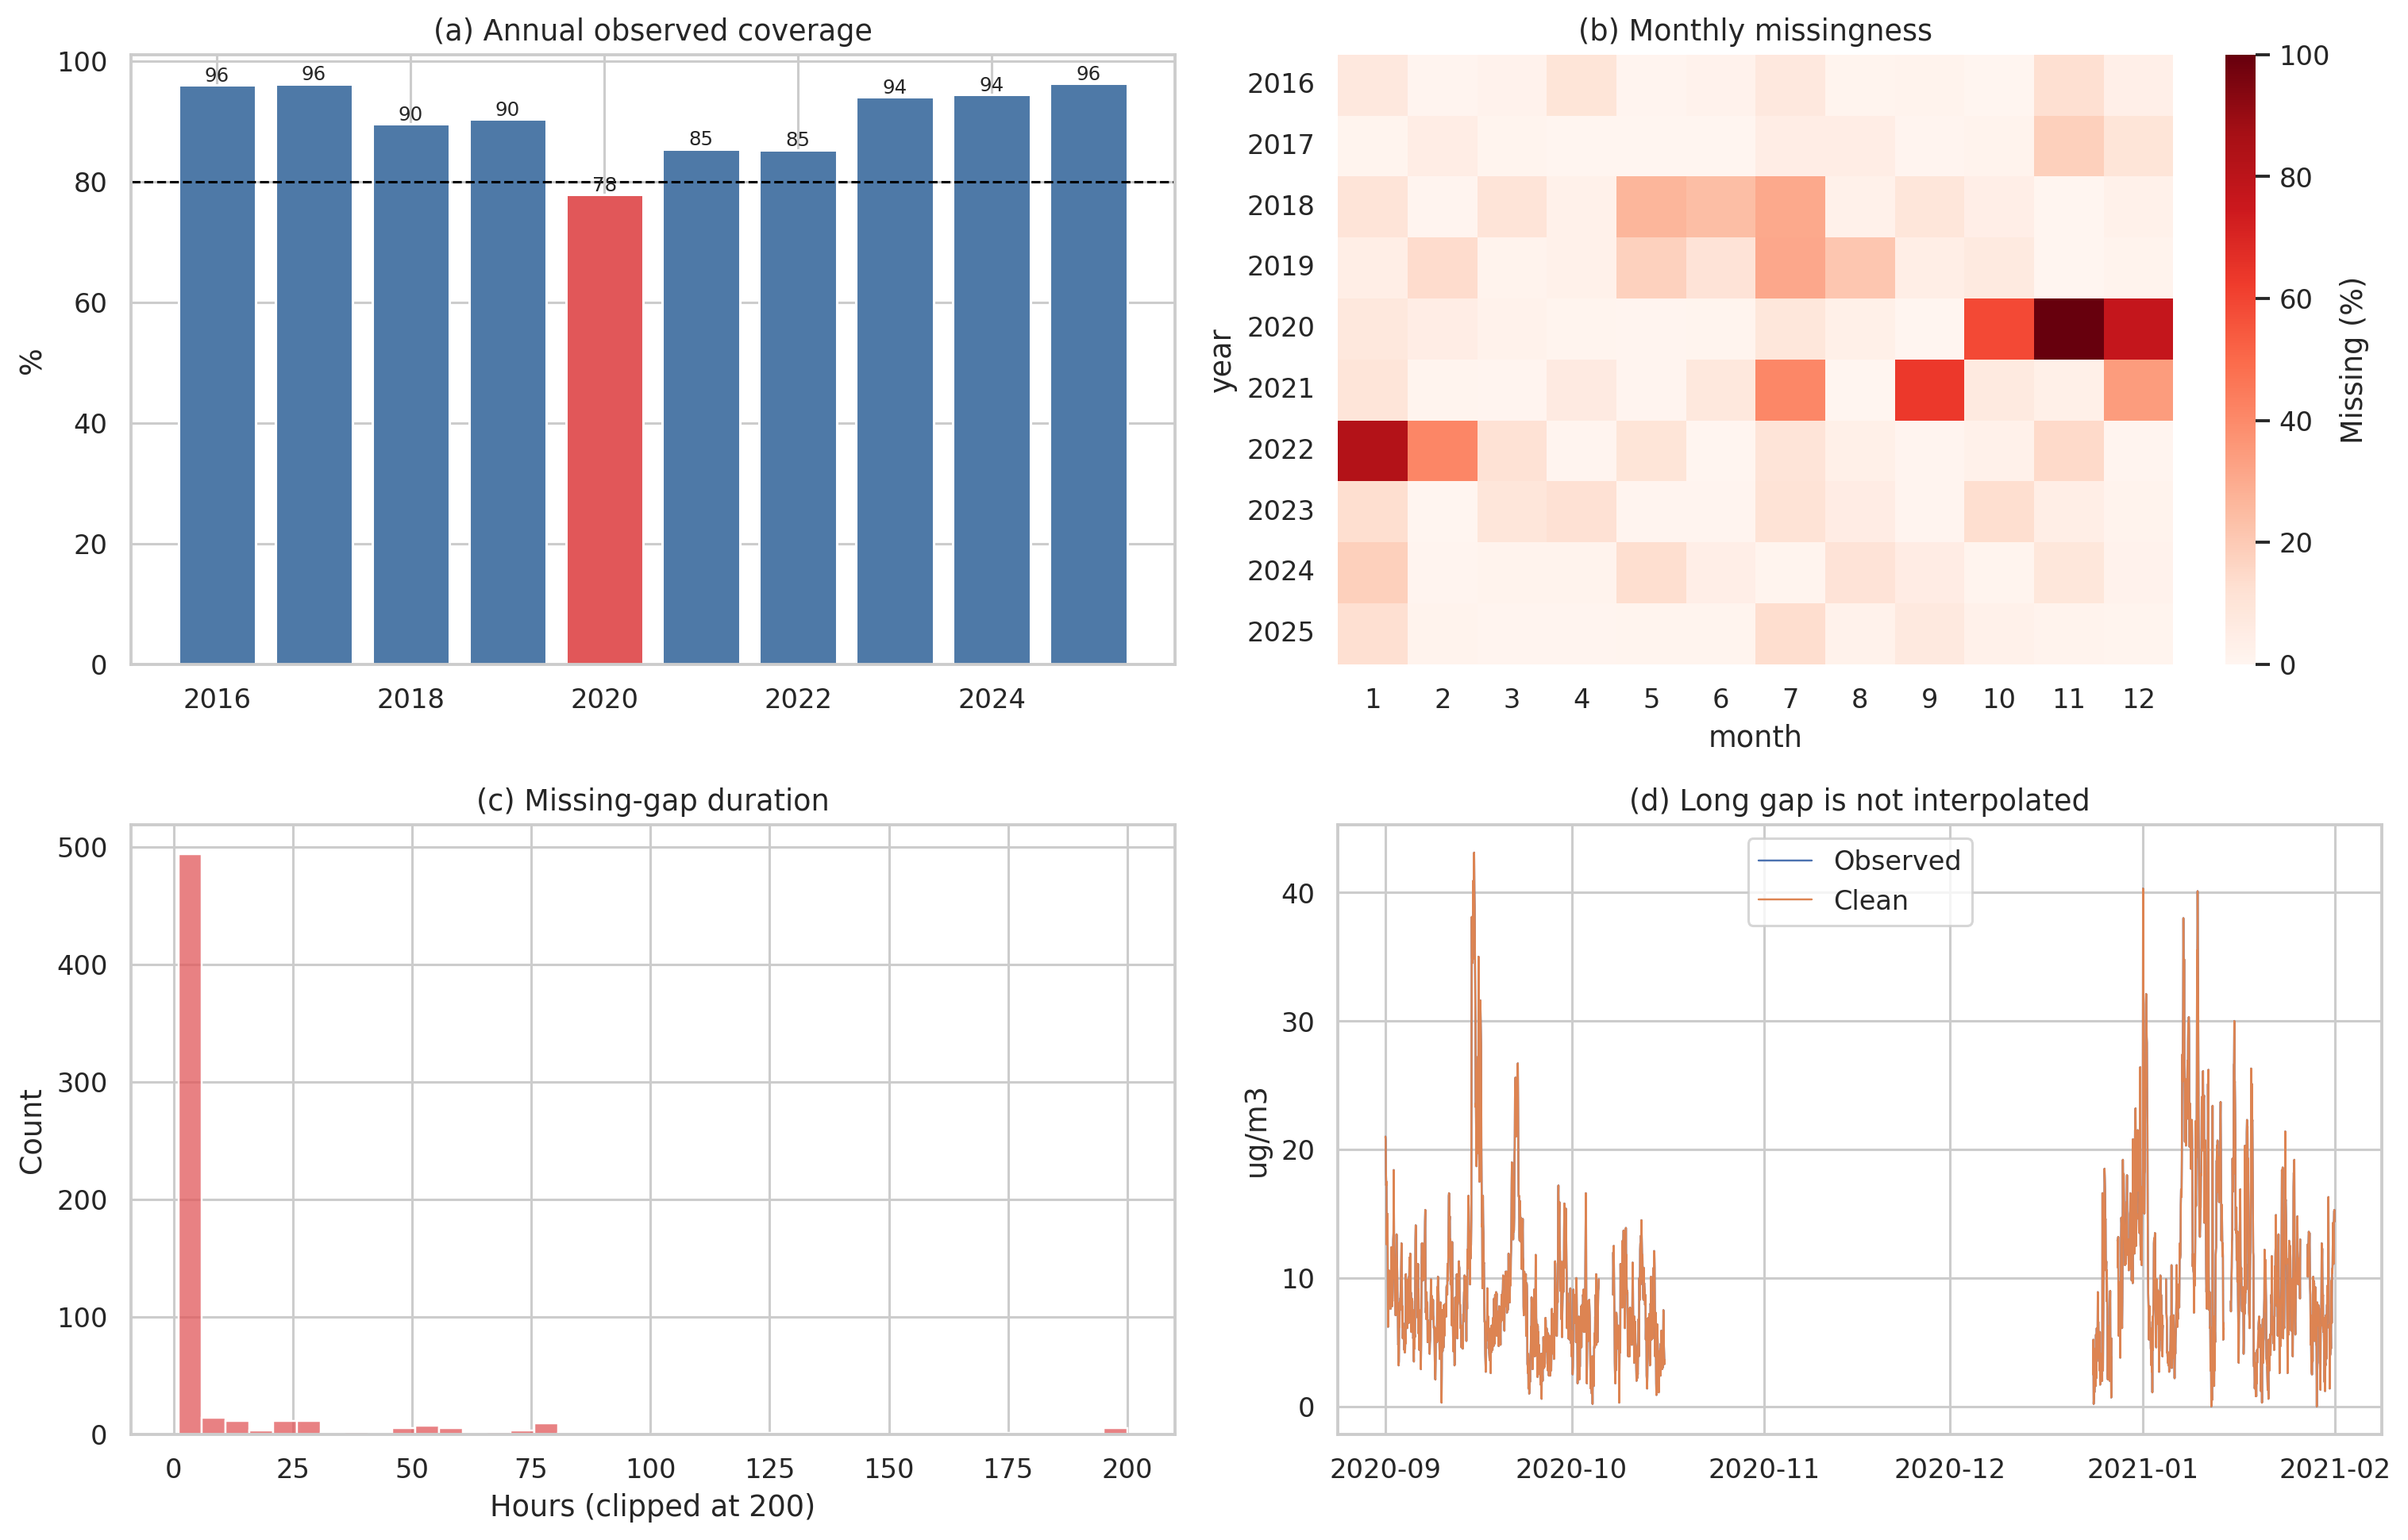
\includegraphics[width=\linewidth]{02_data_quality.png}
\caption{Data-quality audit: coverage, monthly missingness, gap duration, and the preserved long outage.}
\label{fig:data-quality}
\end{figure}}{}

Figure~\ref{fig:data-overview} summarizes the useful temporal signal: PM2.5 is
right-skewed, has repeated daily structure, and remains autocorrelated at
daily and weekly lags. Figure~\ref{fig:data-quality} shows why this structure
cannot be separated from data quality. Coverage changes by year and month, and
long gaps would create artificial trends if interpolated. For this reason, the
main text keeps only two EDA figures; the single-purpose EDA plots are retained
as supplementary outputs generated by the same visualization code.

\IfFileExists{figures/03_multistation_effectiveness.png}{
\begin{figure*}[tbp]
\centering
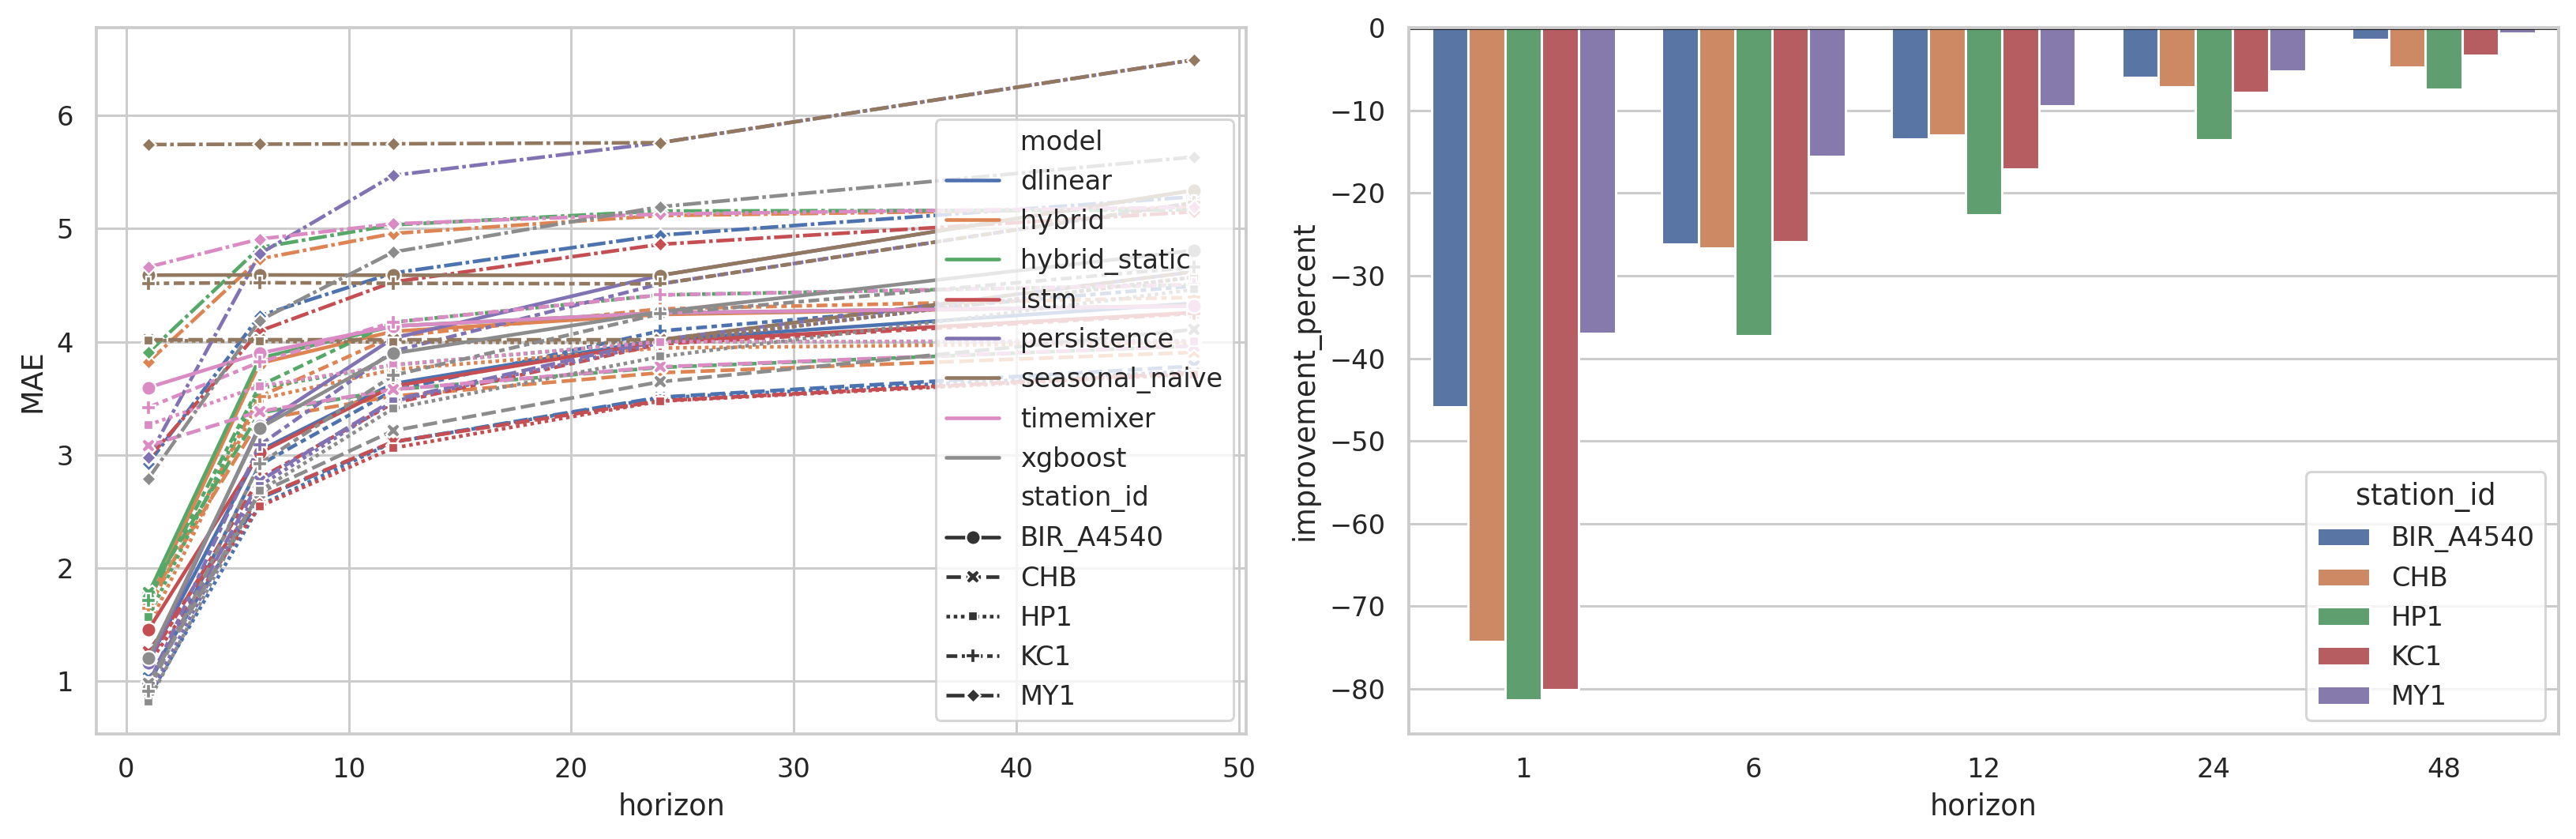
\includegraphics[width=\textwidth]{03_multistation_effectiveness.png}
\caption{Five-seed multi-station effectiveness. Each row compares the hybrid
with the strongest non-hybrid comparator at the same station and horizon; values
below zero mean that the comparator remains better.}
\label{fig:multistation}
\end{figure*}}{}

Figure~\ref{fig:multistation} is the main effectiveness figure. It shows that
the hybrid does not beat the strongest comparator in any of the 25
station-horizon cells. The result exporter accepts only complete gated-v2 runs
covering all five stations, seeds 0--4, and the 30-epoch configuration, so the
reported comparison is not based on a cherry-picked single run. The paper
therefore avoids the phrase ``negative improvement'' in the main interpretation
and reports the result as an MAE gap against stronger baselines.

\IfFileExists{generated_results.tex}{% Auto-generated from complete gated-v2 multi-station results.
\begin{table*}[tbp]
\centering
\caption{Locked-test MAE pooled over station--seed runs. Parentheses show dispersion across both stations and seeds; station-specific comparisons are retained in the machine-readable results.}
\label{tab:multistation-mae}
\begin{tabular}{lrrrrr}
\toprule
Model & 1 h & 6 h & 12 h & 24 h & 48 h \\
\midrule
dlinear & 1.390 (0.791) & 3.070 (0.621) & 3.607 (0.558) & 4.014 (0.537) & 4.329 (0.574) \\
hybrid & 2.070 (0.902) & 3.773 (0.519) & 4.075 (0.502) & 4.264 (0.489) & 4.359 (0.472) \\
hybrid\_static & 2.149 (0.906) & 3.853 (0.531) & 4.144 (0.515) & 4.320 (0.494) & 4.391 (0.460) \\
LSTM & 1.604 (0.708) & \textbf{3.016 (0.578)} & \textbf{3.555 (0.541)} & \textbf{3.959 (0.519)} & \textbf{4.220 (0.536)} \\
persistence & 1.394 (0.816) & 3.324 (0.769) & 4.076 (0.748) & 4.574 (0.655) & 5.251 (0.709) \\
seasonal\_naive & 4.576 (0.645) & 4.577 (0.648) & 4.574 (0.650) & 4.574 (0.655) & 5.251 (0.709) \\
timemixer & 3.605 (0.577) & 3.925 (0.540) & 4.146 (0.518) & 4.316 (0.483) & 4.396 (0.469) \\
XGBoost & \textbf{1.341 (0.751)} & 3.140 (0.576) & 3.804 (0.559) & 4.244 (0.540) & 4.735 (0.519) \\
\bottomrule
\end{tabular}
\end{table*}
The hybrid won 0/25 matched comparisons against the strongest non-hybrid comparator, giving a 23.33\% average MAE gap, while still improving compact TimeMixer.

\begin{table}[tbp]
\centering
\caption{Pooled secondary metrics across all stations, horizons, and seeds. Lower is better for MAE, RMSE, and sMAPE; higher is better for \(R^2\).}
\label{tab:secondary-metrics}
\small
\begin{tabular}{lrrrr}
\toprule
Model & MAE & RMSE & sMAPE & \(R^2\) \\
\midrule
LSTM & \textbf{3.271} & 5.086 & 39.374 & \textbf{0.446} \\
dlinear & 3.282 & \textbf{5.066} & \textbf{39.321} & 0.444 \\
XGBoost & 3.453 & 5.222 & 40.526 & 0.404 \\
hybrid & 3.708 & 5.890 & 43.152 & 0.278 \\
persistence & 3.724 & 5.890 & 43.845 & 0.230 \\
hybrid\_static & 3.771 & 5.940 & 44.049 & 0.268 \\
timemixer & 4.078 & 6.437 & 47.304 & 0.178 \\
seasonal\_naive & 4.710 & 7.477 & 53.853 & -0.104 \\
\bottomrule
\end{tabular}
\end{table}
DLinear and LSTM are practically tied in pooled MAE (3.282 versus 3.271); DLinear leads pooled RMSE and sMAPE.

\begin{table}[tbp]
\centering
\caption{Paired block-bootstrap summary for hybrid minus TimeMixer absolute error. Negative values favor the gated hybrid over its TimeMixer base.}
\label{tab:bootstrap-timemixer}
\small
\begin{tabular}{rrrr}
\toprule
Horizon & Mean diff. & 95\% low & 95\% high \\
\midrule
1 & -1.535 & -1.730 & -1.350 \\
6 & -0.152 & -0.209 & -0.095 \\
12 & -0.071 & -0.120 & -0.023 \\
24 & -0.052 & -0.111 & 0.008 \\
48 & -0.037 & -0.100 & 0.027 \\
\bottomrule
\end{tabular}
\end{table}
Bootstrap evidence supports only the narrower claim that gating helps compact TimeMixer.

\begin{table}[tbp]
\centering
\caption{Common-history sensitivity for the hybrid model. Values are MAE changes after restricting every station to a 2021-start training history; negative values favor the common-history run.}
\label{tab:history-sensitivity}
\begin{tabular}{lrrrr}
\toprule
Grouping & Mean $\Delta$MAE & Median $\Delta$MAE & Improved & Worsened \\
\midrule
All station--horizon cells & 0.012 & 0.019 & 8 & 17 \\
1 h horizons & 0.042 & 0.003 & 1 & 4 \\
6 h horizons & 0.112 & 0.102 & 1 & 4 \\
12 h horizons & 0.014 & 0.042 & 1 & 4 \\
24 h horizons & -0.026 & 0.019 & 2 & 3 \\
48 h horizons & -0.083 & 0.011 & 3 & 2 \\
\bottomrule
\end{tabular}
\end{table}
}{}

The same result files drive the dashboard, which is a research explorer rather
than a live warning service. It exposes station quality, grouped metrics,
residual gates, figures, and explanation panels from completed artifacts.

Table~\ref{tab:multistation-mae} explains which models are strongest by
horizon. \textbf{XGBoost} is strongest at 1 hour, while LSTM and DLinear are
the strongest longer-horizon pair. The difference between their pooled MAE is
only 0.011, so the paper treats them as practically tied rather than crowning
one model from a tiny point estimate. The hybrid improves its intended
TimeMixer base at every horizon, reducing pooled MAE by 42.58\% at 1 hour and
by smaller positive margins from 6 to 48 hours. However, this is a narrower
result than overall superiority: the hybrid pooled MAE is 3.708, compared with
4.078 for TimeMixer, 3.282 for DLinear, and 3.271 for LSTM.

The same-origin ablation separates the TimeMixer base, ungated correction,
static gating, rolling calibration, and reduced-feature variants, isolating
residual fit, over-correction protection, and recent-drift adaptation.

The common-history sensitivity check addresses unequal archive length.
Restricting every station to a 2021-start history changed hybrid MAE by only
\(+0.012~\si{\micro\gram\per\cubic\metre}\) on average across 25 cells: eight
improved and 17 worsened. This changes details but not the conclusion that the
gated hybrid is a TimeMixer calibrator rather than the strongest forecaster.

The ablation identifies over-correction as the ungated learner's main failure
mode. At 12, 24, and 48 hours, ungated MAE reached 6.020, 6.420, and 6.632;
gating reduced them to 4.144, 4.320, and 4.391, with rolling calibration
further reducing them to 4.075, 4.264, and 4.359. The gate selected zero
correction in 56.8\% of fits, so strong correction was supported mainly at short
lead time.

Secondary metrics and bootstrap evidence support the negative finding: RMSE
and sMAPE favor DLinear/LSTM, while paired bootstrap supports only the narrower
claim that gating improves compact TimeMixer. SHAP remains supplementary.
\FloatBarrier

\section{Discussion}
\label{sec:discussion}

Across all station--seed--horizon rows, hybrid MAE was 3.708, compared with 4.078 for compact TimeMixer, 3.282 for DLinear, and 3.271 for LSTM. Thus the gate improves the base model but does not make it globally competitive. The gate selected zero correction in 56.8\% of fits, and common-history sensitivity changed hybrid MAE by only \( +0.012 \), so unequal historical depth does not reverse the conclusion.


\subsection{Interpretation of effectiveness}
\label{sec:discussion-interpretation}

The compact TimeMixer base is weaker than persistence in pooled MAE, so
improving it should not be confused with proving a strong hybrid. At 1 hour,
recent lags support large residual corrections; at longer horizons, the gate
shrinks toward zero as residual predictions become less reliable. This is
useful because unconstrained residual correction caused large negative transfer.
The result also explains why the revised paper avoids a state-of-the-art claim:
the hybrid mechanism is effective as a safety layer over TimeMixer, but the
complete forecasting system is not yet the best model for deployment.

The strongest competing models also clarify the limitation. \textbf{XGBoost}
is best at 1 hour because origin-available lags and rolling statistics almost
directly describe the next-hour state. LSTM and DLinear are nearly tied overall,
which is a useful result in itself: a simple linear decomposition model remains
competitive with a recurrent neural model and both outperform the present
hybrid. In other words, the residual layer repairs some TimeMixer errors, but
it cannot fully compensate for a weak base trajectory. The method is therefore
best interpreted as a controlled residual-calibration lesson rather than a new
state-of-the-art forecaster.

From an application perspective, this is still a useful outcome. A forecasting
system used in environmental monitoring should prefer stable, explainable
performance over architectural novelty. The gated residual layer shows a
practical safeguard: when the calibration set indicates that the residual model
is unreliable, the correction is reduced or disabled. This behavior is easier
to defend than an ungated stacked model that occasionally improves average
scores but produces large horizon-specific failures. The analysis therefore
connects model design with operational reliability, which is one reason the
paper keeps both model-performance tables and data-quality diagnostics in the
main text.

\subsection{Limitations}
\label{sec:discussion-limitations}

Several threats remain. Overlapping windows create serial dependence, five UK
stations do not prove transfer to unseen networks, and station histories differ
(HP1 lacks 2016--2018, BIR\_A4540 begins in 2021, CHB has reduced 2024 coverage,
and KC1 changes instrument regime). The common-history run reduces but does not
eliminate this concern.

The PM2.5-only design also omits forecast-available meteorology, traffic,
co-pollutants, transport patterns, and local events, all of which may matter
during abrupt episodes. Instrument indicators are regime markers, not causal
explanations.

\subsection{Future work}
\label{sec:discussion-future}

Future work should test stronger base forecasters, add only origin-available
external variables, evaluate leave-one-station-out transfer, and compare the
PM2.5-only setting with meteorology-assisted variants under the same locked-test
protocol.

\section{Conclusion and Future Work}
\label{sec:conclusion}

This paper evaluated a gated TimeMixer-XGBoost approach for multi-horizon
hourly PM2.5 forecasting. The study contributes a complete, auditable
forecasting workflow: raw source values are preserved, invalid and negative
measurements are flagged, long gaps are not artificially interpolated, and
features are constructed so that every forecast uses only information
available at its origin. The experimental design covers five monitoring
stations, five forecast horizons, five neural seeds, and a 30-epoch maximum
under chronological training, validation, calibration, and locked-test
partitions.

The main result is mixed but informative. The gated residual layer improves
the compact TimeMixer base at every horizon and greatly reduces the
over-correction seen in ungated residual learning. However, the compact
TimeMixer base is weaker than persistence in pooled MAE, so this improvement
mainly shows that the gate can rescue a weak base, not that the complete hybrid
is superior. The hybrid wins 0 of 25 station-horizon comparisons against the
strongest non-hybrid comparator and has a 23.33\% average MAE gap against that
comparator. LSTM and DLinear are practically tied as the strongest pooled
baselines. The common-history sensitivity analysis supports the same
interpretation: after restricting all stations to a 2021-start history, hybrid
MAE changed by only \(+0.012\) on average across station--horizon cells, so
unequal archive length does not explain away the primary finding.

For a student AI project, this distinction is valuable: the work shows that
simple baselines are competitive, ungated residual stacking can damage
forecasts, and held-out gating is needed when residual evidence is weak. The
next step is to strengthen the base forecaster, add origin-available external
drivers, and test transfer while keeping the same leakage-safe protocol. The
dashboard can later move from artifact explorer to deployed monitoring tool.

Overall, a hybrid architecture should be judged by out-of-sample behavior, not
by complexity. Here, the honest contribution is a leakage-safe negative result
plus a residual-gating lesson: simple baselines remain hard to beat, and a
residual hybrid should first prove that its base forecaster is strong enough to
deserve calibration.

\section*{Data and Code Availability}
The repository contains data-processing and modeling code, tests, figures,
experiment outputs, and manuscript source. UK-Air attribution and licensing
conditions must be preserved.

\section*{Conflict of Interest}
The author declares no conflict of interest.

\begingroup
\small
\bibliographystyle{unsrt}
\bibliography{refs}
\endgroup

\section*{Appendix: Core Notation}
\begin{table}[h]
\centering
\caption{Core notation used in the forecasting formulation.}
\label{tab:notation}
\small
\begin{tabular}{ll}
\toprule
Symbol & Meaning \\
\midrule
$y_t$ & observed hourly PM2.5 at time $t$ \\
$L$ & input history length, fixed at 168 h \\
$\mathcal H$ & direct horizon set $\Horizons$ h \\
$\mathbf{x}_{t-L+1:t}$ & origin-available multichannel sequence \\
$\hat{\mathbf y}^{TM}_t$ & TimeMixer base forecast vector \\
$\mathbf e_t$ & flattened multiscale TimeMixer embedding \\
$\mathbf z_t$ & calendar, instrument, and missingness context \\
$r_{t,h}$ & TimeMixer residual at horizon $h$ \\
$g_h(\cdot)$ & XGBoost residual model for horizon $h$ \\
$\gamma_h$ & held-out calibration correction gate for horizon $h$ \\
\bottomrule
\end{tabular}
\end{table}

\end{document}
